\begin{figure}[t]
    \centering
    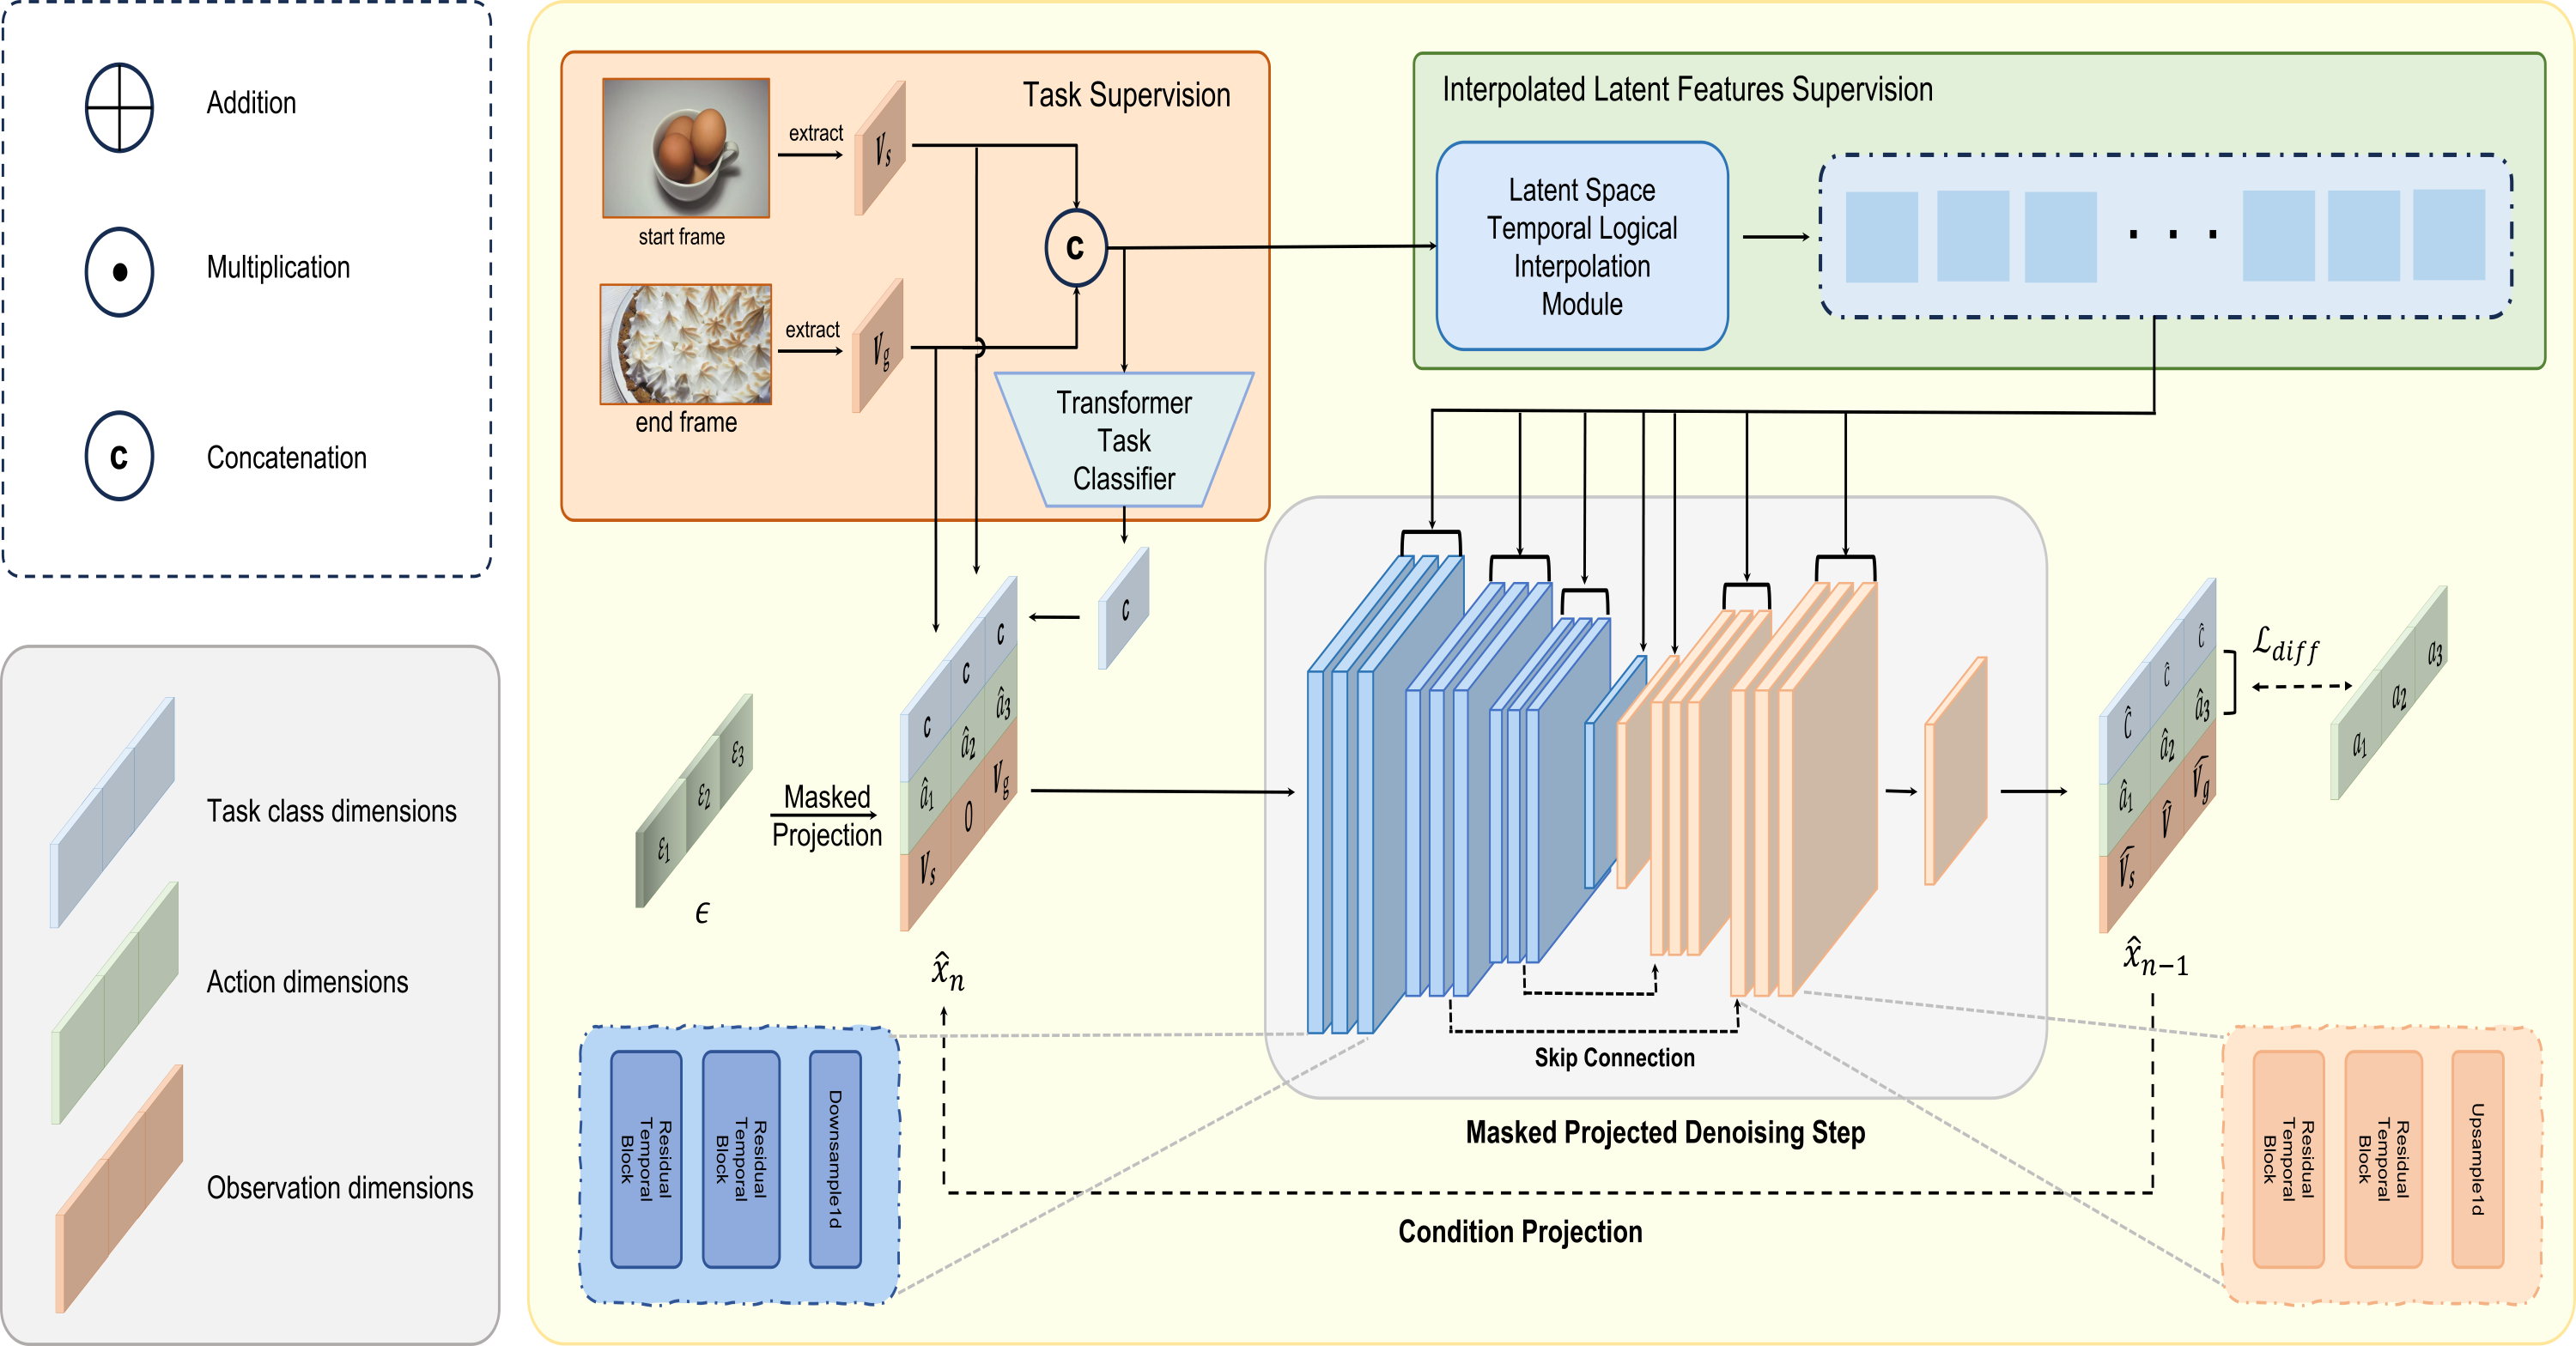
\includegraphics[width=\textwidth,height=0.6\textheight,keepaspectratio]{figures/architecture1.png}
    \caption{Overview of our Masked Temporal Interpolation Diffusion (prediction horizon \( T=3 \)). }
    \label{fig:architecture}
\vspace{-4mm}
\end{figure}
% We first train a transformer task classifier to generate condition information \( c \), which will be used as guidance along with the given observations \( V_s \) and \( V_g \). Subsequently, we put the concatenated observations into the latent space temporal logical interpolation module to obtain the latent temporal logic supervision. Then we compute the denoising process iteratively. In the first step, we conduct a masked projection to the input, then predict the initial distribution by the learned model \( f(\theta) \). We calculate \( \hat{x}_{n-1} \) with the U-Net output \( \hat{x}_0 \). After repeated iterations, we finally select the action dimensions as our result after \( N \) denoising steps.